\documentclass[crop=false]{standalone}

\usepackage[subpreambles=false]{standalone}
\usepackage{import}
\usepackage{graphicx}
\usepackage{subcaption}
\usepackage{tikz}

\begin{document}

\begin{figure*}
  \centering
  % \hspace*{-0.08\linewidth}
  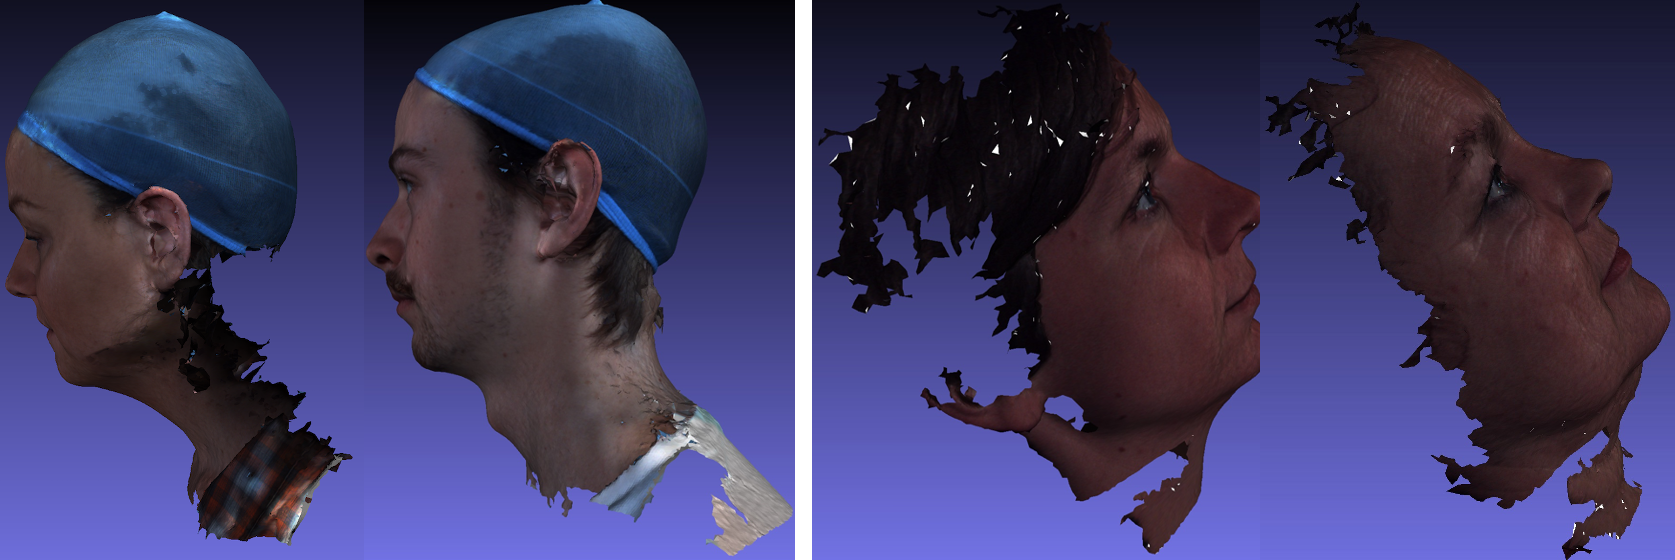
\includegraphics[width=\linewidth]{thesis/methods/import/imgs/data_hs_umc.png}
  %\vspace*{-0.06\linewidth}
  \captionof{figure}{
    \textbf{Data comparison.}
    \small Left: Two subjects from the Headspace data set. Right: Two subjects from the Radboudumc data. The meshes on the right contain more artefacts because a 2-camera setup captured the photos instead of a 5-camera setup. Additionally, the subjects do not wear latex caps which makes the reconstruction of the hair more difficult. The orientation of the Radboudumc meshes is different from that of the Headspace meshes.
  }
  \label{fig:data_hs_umc}
\end{figure*}

\end{document}